\section{Caratteristiche dei sistemi multiagente} \label{sec:sistemi_multiagente}

I sistemi multiagente sono una classe di sistemi composti da un insieme entità autonome, dette agenti, capaci di interagire tra loro e con l'ambiente circostante.
La definizione di agente, come riporta \cite{WooldridgeMichaelJ.1966-2002Aitm}, non è unica e concordata universalmente, ma in generale può essere definito come \textit{un'unità situata in un ambiente, capace di eseguire delle azioni autonome, con la finalità di raggiungere un obiettivo prefissato}.

Un esempio naturale, a cui sono ispirati anche alcuni algoritmi di esplorazione, è rappresentato dalle colonie di formiche: in tali sistemi, migliaia di individui (agenti) agiscono in modo indipendente l'uno dagli altri, collaborando per la ricerca di cibo.
Ciascuna formica prende delle decisioni finalizzate al bene della colonia, basandosi sulla propria visione dell'ambiente che la circonda, e sulle informazioni trasmesse dai suoi simili tramite segnali chimici, come i feromoni.
\begin{figure}[h]
    \centering
    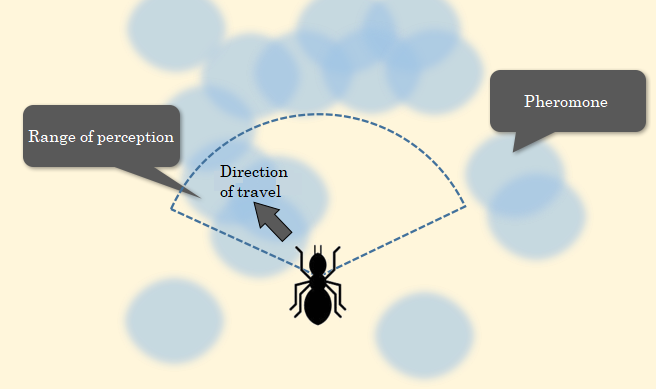
\includegraphics[width=0.6\textwidth]{img/ch1/esempio_formiche_tesi.png}
    \caption{Schema di comportamento di una formica.}
    \label{fig:schema_formica}
\end{figure}

A partire da questo esempio di sistema biologico, è possibile evidenziare alcuni elementi chiave dei sistemi multiagente:
\begin{itemize}

\item \textbf{Obiettivo}:
ogni agente ha un obiettivo e agisce in modo da raggiungerlo.

\item \textbf{Autonomia/Indipendenza}:
ogni agente compie delle scelte e delle azioni in modo autonomo rispetto agli altri agenti del sistema.

\item \textbf{Collaborazione}:
gli agenti possono collaborare tra loro per il raggiungimento di fini comuni nel caso che essi lo ritengano più utile al raggiungimento dell'obiettivo (non tutti i sistemi risultano collaborativi, si immagini per esempio, una partita di poker in cui ogni agente è un giocatore \cite{RussellStuartJ2022Ai:a}).

\item \textbf{Interazione con l'ambiente}:
ogni agente è in grado di interagire con l'ambiente circostante, sia per compiere azioni, sia per raccogliere informazioni propedeutiche alla scelta delle azioni da eseguire.

\item \textbf{Comunicazione}:
gli agenti possono avere dei sistemi per comunicare tra loro, con finalità di coordinazione o di scambio di informazioni.

\end{itemize}

Un'altra caratteristica fondamentale è quella dell' \textbf{ambiente} di essere \textbf{statico o dinamico}: nel primo caso si intende un ambiente che non varia nel tempo, anche a seguito delle azioni degli agenti, mentre per ambiente dinamico si intende un ambiente variabile nel tempo, e che dunque richiede un'analisi continua da parte degli agenti che lo abitano.

L'elenco esposto non è assolutamente esaustivo di tutte le proprietà che permettono la classificazione dei sistemi multiagente e del loro ambiente \cite{RussellStuartJ2022Ai:a}, dato il loro elevato numero si è deciso di evidenziare solo quelle più rilevanti per il caso d'analisi esaminato.

Analogamente all'esempio riportato precedentemente, il sistema multiagente utilizzato in questa tesi è un sistema collaborativo, con obiettivo globale e condiviso tra gli agenti, inserito all'interno di un ambiente parzialmente osservabile e dinamico, che varia sia in modo autonomo, sia a causa dell'azione degli agenti stessi.
